\section{Quasiconvexity and the Weierstra{\ss} Condition}
In \hyperref[sec:mcov_chap2_sec3]{Section 2.3 Extreme Points} we focused on weak local minimizers, i.e. we studied the behaviour of the functional for variations $u=u_*+v$ with $\lVert v\rVert_{C^1(\Omega)}<\varepsilon$, $v\in X_0$ at critical points $u_*$. In particular, $\lVert\nabla v\rVert_{L^\infty(\Omega)}<\varepsilon$. Now we want to study strong local minimizers, i.e. the local behaviour for $u=u_*+v$ with $\lVert v\rVert_{C^0(\Omega)}<\varepsilon$. So $\lVert\nabla v\rVert_{L^\infty(\Omega)}$ is allowed to be arbitrary large.\\

The idea is to consider variations with functions of the form $u=u_*+v_\varepsilon$ with
\[v_\varepsilon(x)=\varepsilon\widetilde{w}\left(\frac{x-x_0}{\varepsilon}\right)\]
so that $\lVert v_\varepsilon\rVert_{L^\infty}=\varepsilon\lVert\widetilde{w}\rVert_{L^\infty}$ is getting smaller and smaller for $\varepsilon\to0$, but $\lVert\nabla v_\varepsilon\rVert_{L^\infty}=\lVert\nabla\widetilde{w}\rVert_{L^\infty}$ can be arbitrary large. The functions $v_\varepsilon$ are suitable for strong local minimizers, but not for weak local minimizers.\\[11pt]

\hypertarget{lemma_2_4_1}{\textbf{Lemma 2.4.1}}\\
Let $f\in C^0(\overline{\Omega}\times\mathbb{R}^m\times\mathbb{R}^{m\times d})$ and $u_*\in C^1(\overline{\Omega};\mathbb{R}^m)$. Let $\widetilde{w}\in C^1(\mathbb{R}^d;\mathbb{R}^m)$ with compact support $\supp{\widetilde{w}}\subset D\subset\mathbb{R}^d$, and set $w(x):=\widetilde{w}\left(\frac{x-x_0}{\varepsilon}\right)$ for some fixed $x_0\in\Omega$. Then
\[\lim_{\varepsilon\searrow0}{\frac{1}{\varepsilon^d}\left(I(u_*+\varepsilon w)-I(u_*)\right)}=\int_D{f(x_0,u_*(x_0),\nabla u_*(x_0)+\nabla\widetilde{w}(y))-f(x_0,u_*(x_0),\nabla u_*(x_0))\mathrm{d}y}.\]\\

\textit{Proof:}\\
Choose $\varepsilon>0$ so small that $x_0+\varepsilon D\subset\Omega$. Then the boundary terms coming from $I$ vanish and we get
\begin{align*}
	\frac{1}{\varepsilon^d}(I(u_*+\varepsilon w)-I(u_*))&=\frac{1}{\varepsilon^d}\int_{x_0+\varepsilon D}{f\left(x,u_*(x)+\varepsilon\widetilde{w}\left(\frac{x-x_0}{\varepsilon}\right),\nabla u_*(x)+\nabla\widetilde{w}\left(\frac{x-x_0}{\varepsilon}\right)\right)\mathrm{d}x}\\
	&\qquad\qquad-\frac{1}{\varepsilon^d}\int_{x_0+\varepsilon D}{f(x,u_*(x),\nabla u_*(x))\mathrm{d}x}\\
	&=\int_D{f(x_0+\varepsilon y,u_*(x_0+\varepsilon y)+\varepsilon\widetilde{w}(y),\nabla u_*(x_0+\varepsilon y)+\nabla\widetilde{w}(y))\mathrm{d}y}\\
	&\qquad\qquad-\int_D{f(x_0+\varepsilon y,u_*(x_0+\varepsilon y),\nabla u_*(x_0+\varepsilon y))\mathrm{d}y}.
\end{align*}
Now we can use Lebesgue's dominated convergence theorem by uniform continuity of $f$ and $u_*$ on compact sets.\hfill$\blacksquare$\\[11pt]

\hypertarget{definition_2_4_2}{\textbf{\underline{Definition 2.4.2}}}\\
(Quasiconvexity, Money, 1952)\\
A function $\tilde{f}\in C^0(\mathbb{R}^{m\times d};\mathbb{R})$ is called \textit{quasiconvex in a point $A\in\mathbb{R}^{m\times d}$} if
\begin{align}\label{eq:mcov_formula_qc}
	\int_D{\tilde{f}(A+\nabla\widetilde{w}(y))\mathrm{d}y}\geq\int_D{\tilde{f}(A)\mathrm{d}y}=\tilde{f}(A)\vol{D}\tag{QC}
\end{align}
for all domains $D\subset\mathbb{R}^d$, all test functions $\widetilde{w}\in C^1(\mathbb{R}^d;\mathbb{R}^m)$ with compact support $\supp{\widetilde{w}}\subset D$.\\

If $\tilde{f}$ is quasiconvex in every point, then $\tilde{f}$ is called \textit{quasiconvex}.\newpage

\textbf{Remark 2.4.3}\\
The definition of quasiconvexity is somehow complicated to verify and unnatural. However, one can show that quasiconvexity does not depend on the choice of $D$, i.e. if \eqref{eq:mcov_formula_qc} is satisfied for one domain $D$, e.g. $D=B_1(0)$, then \eqref{eq:mcov_formula_qc} holds for all domains.\\[11pt]

\hypertarget{theorem_2_4_4}{\textbf{\underline{Theorem 2.4.4}}}\\
(Quasiconvexity as necessary condition)\\
Let $f\in C^0(\Omega\times\mathbb{R}^m\times\mathbb{R}^{m\times d})$. If $u_*\in C^1(\overline{\Omega};\mathbb{R}^m)$ is a strong local minimizer of $I$, then the mapping $A\longmapsto f(x_0,u_*(x_0),A)$ is quasiconvex in $A=\nabla u_*(x_0)$ for all $x_0\in\Omega$.\\

\textit{Proof:}\\
Assume that $A\longmapsto f(x_0,u_*(x_0),A)$ is not quasiconvex in $A=\nabla u_*(x_0)$ for some $x_0\in\Omega$. Then there are $D$, $\widetilde{w}$ as in \hyperlink{definition_2_4_2}{Definition 2.4.2} such that
\[\int_D{f(x_0,u_*(x_0),\nabla u_*(x_0)+\nabla\widetilde{w}(y))\mathrm{d}y}<\int_D{f(x_0,u_*(x_0),\nabla u_*(x_0))\mathrm{d}y}.\]
Define $w(x):=\widetilde{w}\left(\frac{x-x_0}{\varepsilon}\right)$. \hyperlink{lemma_2_4_1}{Lemma 2.4.1} provides
\begin{align*}
	&\frac{1}{\varepsilon^d}\left(I(u_*+\varepsilon w)-I(u_*)\right)\\
	&\qquad\qquad=\int_D{f(x_0,u_*(x_0),\nabla u_*(x_0)+\nabla\widetilde{w}(y))-f(x_0,u_*(x_0),\nabla u_*(x_0))\mathrm{d}y}+o(1).
\end{align*}
So if $\varepsilon$ is small then $I(u_*+\varepsilon w)-I(u_*)<0$ which is a contradiction to the minimizing property of $u_*$.\hfill$\blacksquare$\\[11pt]

The idea is that if we have a list of critical points we could check which of them satisfy the quasiconvexity condition from \hyperlink{theorem_2_4_4}{Theorem 2.4.4} to shrink the list of candidates. But quasiconvexity is a global condition containing an integral, thus it is difficult to verify it in practice. We next derive a local/pointwise condition, the so-called Weierstra{\ss} condition.\\[11pt]

\hypertarget{theorem_2_4_5}{\textbf{\underline{Theorem 2.4.5}}}\\
(Weierstra{\ss}' necessary condition)\\
Let $f\in C^1(\Omega\times\mathbb{R}^m\times\mathbb{R}^{m\times d})$. If $u_*\in C^1(\overline{\Omega};\mathbb{R}^m)$ is a strong local minimizer of $I$, then it holds
\[f(x,u_*(x),\nabla u_*(x)+\xi\otimes\eta)-f(x,u_*(x),\nabla u_*(x))-D_Af(x,u_*(x),\nabla u_*(x))[\xi\otimes\eta]\geq0\]
for all $x\in\Omega$, $\xi\in\mathbb{R}^m$, $\eta\in\mathbb{R}^d$.\\[11pt]

\textbf{Remark 2.4.6}
\begin{itemize}
	\item[(a)] If $f$ is even a $C^2$-function, we can set $\xi=\alpha\tilde{\xi}$ and use a Taylor expansion with respect to $\alpha$ to obtain the Legendre-Hadamard condition $D_A^2f(x,u(x),\nabla u(x))[\tilde{\xi}\otimes\eta]\geq0$.
	\item[(b)] $E(x,u,A,\xi,\eta)=f(x,u,A+\xi\otimes\eta)-f(x,u,A)-D_Af(x,u,A)[\xi\otimes\eta]$ is called the \textit{Weierstra{\ss} excess function}.
	\item[(c)] Weierstra{\ss} only considered the case $d=1$. Then $\eta$ can be dropped in the excess function,
	\[E(x,u,A,\xi)=f(x,u,A+\xi)-\underbrace{[f(x,u,A)+\partial_Af(x,u,A)\cdot\xi]}_{\substack{\text{geometrically the tangent line}\\\text{to }f(x,u,\cdot)\text{ at }A}}.\]
	Along strong local minimizer, $f$ \glqq exceeds\grqq{} its tangent lines. Recall \hyperlink{example_2_3_3}{Example 2.3.3}.

	\begin{figure}[ht]
		\centering
		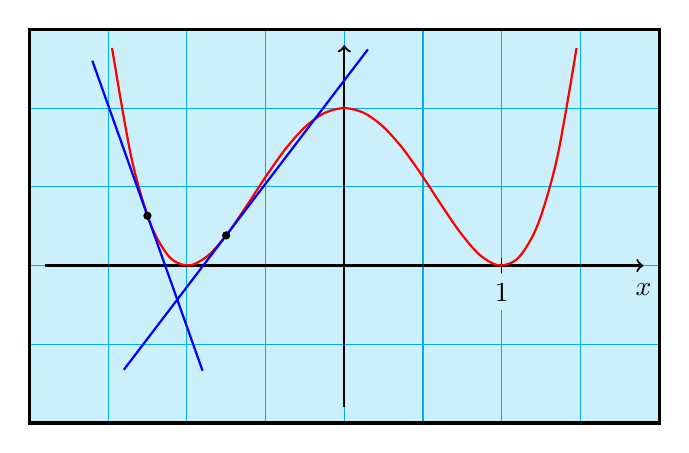
\begin{tikzpicture}
			% Hintergrund
			\fill[cyan!20] (-4, -2) rectangle (4, 3);
			\draw[cyan, step=1] (-4, -2) grid (4, 3);

			% Achsen
			\draw[thick, ->] (-3.8, 0) -- (3.8, 0);
			\node at (3.8, -0.3) {$x$};
			\draw[thick, ->] (0, -1.8) -- (0, 2.8);
			\draw[thin] (2, 0.1) -- (2, -0.1) node[below, fill=cyan!20] {$1$};

			% Funktionen
			\draw[thick, red] plot[smooth, domain=-2.95:2.95] (\x, {2*(1-(\x/2)^2)^2});
			\draw[thick, blue] plot[smooth, domain=-3.2:-1.8] (\x, {0.6328125-2.8125*(\x+2.5)});
			\fill (-2.5, 0.6328125) circle (1.5pt);
			\draw[thick, blue] plot[smooth, domain=-2.8:0.3] (\x, {0.3828125+1.3125*(\x+1.5)});
			\fill (-1.5, 0.3828125) circle (1.5pt);

			% Rahmen
			\draw[very thick] (-4, -2) rectangle (4, 3);
		\end{tikzpicture}
		\caption{Volume density $f$ with tangent lines.}
		\label{fig:remark_2_4_6}
	\end{figure}

	From \hyperref[fig:remark_2_4_6]{Figure II.6} we obtain $E\geq0$ in $(-\infty,-1]\cup[1,\infty)$, but $E<0$ in $(-1,1)$ for some values $\xi\in\mathbb{R}$.\\

	In 1D, the condition $E(x,u,A,\xi)\geq0$ for all $\xi\in\mathbb{R}^m$ is equivalent to convexity and to quasiconvexity of $A\longmapsto f(x,u,A)$.\\[11pt]
\end{itemize}

\textit{Proof of \hyperlink{theorem_2_4_5}{Theorem 2.4.5}}\\
We construct a suitable test function $\widetilde{w}$ with $\nabla\widetilde{w}=\xi\otimes\eta$. For that, we will define a certain function $\alpha\in C^1(\mathbb{R}^d;\mathbb{R})$ and put $\widetilde{w}(y)=\alpha(y)\xi\in\mathbb{R}^m$. Then $\nabla\widetilde{w}(y)=\xi\otimes\nabla\alpha(y)$.\\

\textit{Step 1:} Special case $\eta=(\eta_1,0,\dotsc,0)^\top\in\mathbb{R}^d$ with $\eta_1\geq0$.
\begin{itemize}
	\item[] We write $y=(y_1,\hat{y})\in\mathbb{R}^d$ with $y_1\in\mathbb{R}$, $\hat{y}\in\mathbb{R}^{d-1}$. Let $\mathcal{C}\subset B_1(0)$ be a cone with flat base $\{y\in\mathbb{R}^d\mid y_1=\frac{1}{2},\lvert\hat{y}\rvert\leq\frac{1}{2}\}$ and vertex $(\frac{1}{2}-\delta,0,\dotsc,0)\in\mathbb{R}^d$, where $0<\delta<\frac{1}{2}$. The mantle is given by $\{(y_1,\hat{y})\mid y_1=\frac{1}{2}-\beta(\hat{y})\}$ with $\beta(\hat{y})=\delta(1-2\lvert\hat{y}\rvert)$. Set
	\[\alpha(y)=\left\{\begin{array}{rl}
		0&\text{for }\lvert\hat{y}\rvert\geq\frac{1}{2}\text{ or }\lvert y_1\rvert\geq\frac{1}{2},\\
		\lvert\eta\rvert(y_1-\frac{1}{2})&\text{for }y_1\in\left[\frac{1}{2}-\beta(\hat{y}),\frac{1}{2}\right],\\
		\frac{-\lvert\eta\rvert\beta(\hat{y})}{1-\beta(\hat{y})}\left(y_1+\frac{1}{2}\right)&\text{for }y_1\in\left[-\frac{1}{2},\frac{1}{2}-\beta(\hat{y})\right].
	\end{array}\right.\]

	\begin{figure}[ht]
		\centering
		\begin{tikzpicture}
			% Achsen
			\draw[thick, ->] (-3, 0) -- (3, 0) node[right] {$\hat{y}$};
			\draw[thick, ->] (0, -2.5) -- (0, 2.5) node[right] {$y_1$};

			% Flächenmarkierungen im Koordinatensystem
			\fill[pattern={Lines[angle=-45, distance=1mm]}, pattern color=red] circle (2);
			\fill[white] (-1, -1) rectangle (1, 1);
			\draw[thick] (-1, 0) -- (1, 0) (0, -1) -- (0, 1);
			\fill[pattern={Dots}, pattern color=olive] (-1, 1) -- (-1, -1) -- (1, -1) -- (1, 1) -- (0, 0.2) -- (-1, 1);
			\fill[pattern={Lines[angle=45, distance=1mm]}, pattern color=yellow] (-1, 1) -- (1, 1) -- (0, 0.2) -- (-1, 1);

			% Zeichnungen im Koordinatensystem
			\draw circle (2);
			\draw[dashed] (-1, 1) -- (-1, -1) -- (1, -1) -- (1, 1);
			\draw (-1, 1) -- (1, 1) -- (0, 0.2) -- (-1, 1);
			\draw[thin] (-0.1, 0.2) -- (0.1, 0.2);

			% Beschriftungen
			\draw[thin] (-2, 0.1) -- (-2, -0.1);
			\draw[thin] (2, 0.1) -- (2, -0.1);
			\node at (-2.3, -0.3) {$-1$};
			\node at (2.1, -0.3) {$1$};
			\fill[white] (0.25, 0.04) rectangle (0.9, 0.36);
			\node at (0.55, 0.2) {\scriptsize$\frac{1}{2}-\delta$};
		\end{tikzpicture}
		\caption{Illustration of $\mathcal{C}$ in $\mathbb{R}^2$ and piecewise definition of $\alpha$.}
	\end{figure}

	By definition, $\supp{\alpha}\subset B_1(0)$, $\nabla\alpha(y)=\lvert\eta\rvert e_1=\eta$ for $y\in\mathcal{C}$ and $\nabla\alpha(y)=O(\delta)$ for $y\notin\mathcal{C}$. Moreover, $\alpha$ is Lipschitz continuous, but not necessarily differentiable everywhere. So we approximate $\alpha$ by $C^1$-functions in a neighbourhood of the kinks and use $\widetilde{w}(y)=\alpha(y)\xi$ in the quasiconvexity condition (and make use of \hyperlink{theorem_2_4_4}{Theorem 2.4.4})
	\begin{align*}
		0&\leq\int_{B_1(0)}{f(x,u,A+\nabla\widetilde{w}(y))-f(x,u,A)\mathrm{d}y}\\
		&=\int_\mathcal{C}{f(x,u,A+\xi\otimes\eta)-f(x,u,A)\mathrm{d}y}+\int_{B_1(0)\setminus\mathcal{C}}{\left[D_Af(x,u,A)[\nabla\widetilde{w}(y)]+o(\delta)\right]\mathrm{d}y}\\
		&=(f(x,u,A+\xi\otimes\eta)-f(x,u,A))\int_\mathcal{C}{1\mathrm{d}y}\\
		&\qquad\qquad+D_Af(x,u,A):\left[\int_{B_1(0)\setminus\mathcal{C}}{\xi\otimes\nabla\alpha(y)\mathrm{d}y}\right]+o(\delta).
	\end{align*}
	Gau{\ss} theorem implies
	\[\int_{B_1(0)\setminus\mathcal{C}}{\nabla\alpha(y)\mathrm{d}y}=\int_{B_1(0)}{\nabla\alpha(y)\mathrm{d}y}-\int_\mathcal{C}{\nabla\alpha(y)\mathrm{d}y}=0-\int_\mathcal{C}{\eta\mathrm{d}y}.\]
	Hence
	\[0\leq\left(f(x,u,A+\xi\otimes\eta)-f(x,u,A)-D_Af(x,u,A)[\xi\otimes\eta]\right)\underbrace{\int_\mathcal{C}{1\mathrm{d}y}}_{=c\cdot\delta}+o(\delta),\]
	i.e.
	\[0\leq f(x,u,A+\xi\otimes\eta)-f(x,u,A)-D_Af(x,u,A)[\xi\otimes\eta]+o(1)\]
	as $\delta\to0$.\\
\end{itemize}

\textit{Step 2:} General case.
\begin{itemize}
	\item[] By rotating the coordinate system, we can reduce the general case to step 1. So we assume $\eta=(\eta_1,\dotsc,\eta_d)$ is arbitrary, then there exists a rotation matrix $R\in\mathbb{R}^{d\times d}$ such that $R\eta=\overline{\eta}:=(\lvert\eta\rvert,0,\dotsc,0)$. Then let $\alpha$ be the function constructed in step 1. with respect to $\overline{\eta}$ and define $\overline{\alpha}(y)=\alpha(Ry)$. For $\overline{y}=R^{-1}y\in R^{-1}\mathcal{C}$ we then have
	\[\nabla_{\overline{y}}\overline{\alpha}(\overline{y})=\nabla_{\overline{y}}\alpha(R\overline{y})=\nabla_y\alpha(y)\cdot R=\overline{\eta}^\top\cdot R=\eta^\top.\]
	Hence, by replacing $\alpha$ with $\overline{\alpha}$ and $\mathcal{C}$ with $R^{-1}\mathcal{C}$ in the computations in step 1., we get the same result since $\vol{\mathcal{C}}=\vol{R^{-1}\mathcal{C}}$.\hfill$\blacksquare$\\[11pt]
\end{itemize}

\textbf{\underline{Theorem 2.4.7}}\\
(Weierstra{\ss}'s sufficient condition)\\
Let $\Omega=(\alpha,\beta)\subset\mathbb{R}^1$, $I(u)=\int_\alpha^\beta{f(x,u(x),u'(x))\mathrm{d}x}$, and let $u_*\in C_0^1([\alpha,\beta];\mathbb{R}^m)$ be a weak local minimizer. Suppose that
\begin{itemize}
	\item[(i)] there exists $\gamma_*>0$ such that
	\[D^2I(u_*)[v]\geq\gamma_*\int_\alpha^\beta{\lvert v'(x)\rvert^2+\lvert v(x)\rvert^2\mathrm{d}x}\]
	for all $v\in C_0^1([\alpha,\beta];\mathbb{R}^m)$, and
	\item[(ii)] there exists $\varepsilon>0$ such that for all $x\in[\alpha,\beta]$, $\tilde{u},\tilde{A}\in\mathbb{R}^m$ with $\lvert\tilde{u}-u_*(x)\rvert<\varepsilon$ and $\lvert\tilde{A}-u_*'(x)\rvert<\varepsilon$ it holds $E(x,\tilde{u},\tilde{A},B)\geq0$ for all $B\in\mathbb{R}^m$.
\end{itemize}
Then $u_*$ is a strict strong local minimizer.\\

\textit{Remark: With the first condition we are already familiar, cf. \hyperlink{theorem_2_3_4}{Theorem 2.3.4}. And in the second condition, the exceed function comes in.}\\

\textit{Proof:}\\
The proof of this theorem opens a whole new theory and is quite complicated. See \cite[Chapter ?, Section ? Theorem ?]{magnus_r_hestenes}.\hfill$\blacksquare$\\[11pt]

A common and easy assumption which guarantees existence is the standard convexity. Next, we will collect some different notions of convexity.\\[11pt]

\hypertarget{definition_2_4_8}{\textbf{\underline{Definition 2.4.8}}}\\
Let $\tilde{f}:\mathbb{R}^{m\times d}\longrightarrow\mathbb{R}$ and $A_0\in\mathbb{R}^{m\times d}$.
\begin{itemize}
	\item[(i)] $\tilde{f}$ is called \textit{convex in $A_0$} if there exists $B\in\mathbb{R}^{m\times d}$ such that
	\[\tilde{f}(A_0+C)\geq\tilde{f}(A_0)+B:C\]
	for all $C\in\mathbb{R}^{m\times d}$.
	\item[(ii)] $\tilde{f}$ is called \textit{quasiconvex in $A_0$} if for all $w\in C_0^1(B_1(0);\mathbb{R}^m)$
	\[\frac{1}{\vol{B_1(0)}}\int_{B_1(0)}{\tilde{f}(A_0+\nabla w(x))\mathrm{d}x}\geq\tilde{f}(A_0)\]
	\item[(iii)] $\tilde{f}$ is called \textit{rank-one convex in $A_0$} if there exists $B\in\mathbb{R}^{m\times d}$ such that
	\[\tilde{f}(A_0+\xi\otimes\eta)\geq\tilde{f}(A_0)+B:(\xi\otimes\eta)\]
	for all $\xi\in\mathbb{R}^m$, $\eta\in\mathbb{R}^d$.
\end{itemize}
Moreover, $\tilde{f}$ is called \textit{convex} / \textit{quasiconvex} / \textit{rank-one convex} if $\tilde{f}$ is convex / quasiconvex /rank-one convex in every point $A_0\in\mathbb{R}^{m\times d}$.\newpage

\textbf{Remark 2.4.9}
\begin{itemize}
	\item[(a)] $\tilde{f}$ is convex if and only if for all $A_1,A_2\in\mathbb{R}^{m\times d}$ it holds
	\begin{align}\label{eq:mcov_formula_c}
		\tilde{f}((1-\lambda)A_1+\lambda A_2)\leq(1-\lambda)\tilde{f}(A_1)+\lambda\tilde{f}(A_2)\tag{C}
	\end{align}
	for all $\lambda\in(0,1)$.
	\item[(b)] $\tilde{f}$ is rank-one convex if and only if (C) holds for all $A_1,A_2\in\mathbb{R}^{m\times d}$ such that $A_1-A_2$ has rank 1, i.e. $A_1-A_2=\xi\otimes\eta$ for some $\xi\in\mathbb{R}^n$, $\eta\in\mathbb{R}^d$.\\[11pt]
\end{itemize}

\hypertarget{theorem_2_4_10}{\textbf{\underline{Theorem 2.4.10}}}\\
Let $\tilde{f}:\mathbb{R}^{m\times d}\longrightarrow\mathbb{R}$ and $A_0\in\mathbb{R}^{m\times d}$. Then the following implications hold:
\[\tilde{f}\text{ convex in }A_0\quad\Rightarrow\quad\tilde{f}\text{ quasiconvex in }A_0\quad\Rightarrow\quad\tilde{f}\text{ rank-one convex in }A_0.\]
If $m=1$ or $d=1$, then $\tilde{f}$ is convex in $A_0$ if and only if it is rank-one convex in $A_0$.\\[11pt]

\textbf{Remark 2.4.11}\\
How about the other implications?
\begin{itemize}
	\item[(a)] Morrey conjectured 1952/1966, that quasiconvexity does not imply rank-one convexity.
	\item[(b)] In 1992, \v{S}ver\'ak showed for the case $m\geq3$, $d\geq2$ the existence of an analytic function $\tilde{f}:\mathbb{R}^{m\times d}\longrightarrow\mathbb{R}$ that is rank-one convex but not quasiconvex. However, the case $d=2$ or $m=2$ is still an open problem.
	\item[(c)] Quasiconvexity does not imply convexity, for example consider $\tilde{f}(A)=\det(A)$.\\
\end{itemize}

\textit{Proof of \hyperlink{theorem_2_4_10}{Theorem 2.4.10}:}
\begin{itemize}
	\item[(i)] First we show that convexity implies quasiconvexity. By definition, there exists $B\in\mathbb{R}^{m\times d}$ such that $\tilde{f}(A_0+C)\geq\tilde{f}(A_0)+B:C$ for all $C\in\mathbb{R}^{m\times d}$. Apply this pointwise to $C=\nabla w(y)$ for $w\in C_0^1(B_1(0);\mathbb{R}^m)$ with $y\in B_1(0)$. Then
	\begin{align*}
		\int_{B_1(0)}{\tilde{f}(A+\nabla w(y))\mathrm{d}y}&\geq\int_{B_1(0)}{\tilde{f}(A_0)+B:\nabla w(y)\mathrm{d}y}\\
		&=\tilde{f}(A_0)\vol{B_1(0)}+B:\underbrace{\int_{B_1(0)}{\nabla w(y)\mathrm{d}y}}_{=0}
	\end{align*}
	because
	\[\int_{B_1(0)}{(\nabla w(y))_{ij}\mathrm{d}y}=\int_{B_1(0)}{\frac{\partial}{\partial y_j}w_i(y)\mathrm{d}y}=\int_{\partial B_1(0)}{w_i(y)\nu_j(y)\mathrm{d}a}=0.\]
	\item[(ii)] For the direction from quasiconvexity to rank-one convexity one can proceed as in the proof for Weierstra{\ss}' necessary condition, \hyperlink{theorem_2_4_5}{Theorem 2.4.5}.
	\item[(iii)] Assume $\tilde{f}$ is rank-one convex and $\min\{m,d\}=1$. Then each arbitrary $C\in\mathbb{R}^{m\times d}$ has always the form $C=\xi\otimes\eta$ with $\xi\in\mathbb{R}^m$, $\eta\in\mathbb{R}^d$. Thus, convexity holds.\hfill$\blacksquare$
\end{itemize}